\chapter{行动顺序与乱敏机制}

行动顺序是石器时代战斗体验中最显性的结果之一，但它并不是一个“谁敏高谁先手”的静态比较，而是一个由参照敏捷、动作类型、骑宠混合和随机扰动共同决定的排序过程。本章的重点不是重复“乱敏存在”这一常识，而是把乱敏写成可分析的分段模型，并说明哪些技能真正吃骑宠混合敏，哪些技能其实只看人物自己的速度敏。

\section{普通行动的乱敏公式}

当前源码里，大多数普通行动都先取一个参照敏捷 $Q_{\mathrm{ref}}$，再把它写成
\begin{equation}
    w = Q_{\mathrm{ref}} + 20,
\end{equation}
最后生成顺序值
\begin{equation}
    S_{\mathrm{normal}} = w - \operatorname{RAND}(0,0.3w).
    \label{eq:turn-normal}
\end{equation}
式~\eqref{eq:turn-normal} 就是玩家口中的“乱敏”。它的含义不是“敏捷有一点随机误差”，而是顺序值会在区间
\begin{equation}
    S_{\mathrm{normal}} \in [0.7w,\; w]
\end{equation}
内波动。也就是说，敏捷优势并不会被完全抹平，但只要双方区间存在重叠，就仍有可能发生逆转。

道具使用与迅速类动作在这一基础上另有修正。道具顺序值可整理为
\begin{equation}
    S_{\mathrm{item}} = w - \operatorname{RAND}(0,0.3w) + 0.15w,
    \label{eq:turn-item}
\end{equation}
也就是在普通乱敏基础上再加 $15\%$。迅速攻击类则更激进，直接写成
\begin{equation}
    S_{\mathrm{quick}} = w + 0.3w = 1.3w,
    \label{eq:turn-quick}
\end{equation}
当前实现中这一段没有再附带随机扣减，因此它更像一个确定性的速度档提升，而不是“更高敏也照样大乱”的动作。

\section{道具、迅速行动与职业技能速度档}

从实现结构看，速度档并不只由“动作中文名”决定，而是由动作最终进入 \code{BATTLE_DexCalc()} 时走哪一条分支决定。最基础的一类是前节的默认档，即式~\eqref{eq:turn-normal}。第二类是物品档，即式~\eqref{eq:turn-item}。第三类是迅速档，即式~\eqref{eq:turn-quick}。除此以外，职业技能还会出现若干只看人物 \code{WORKQUICK} 的专用公式。

对于职业技能，最关键的区分是“该技能是否沿用默认档”。若沿用默认档，则其参照敏捷可能是人物敏，也可能是骑宠混合敏；若进入技能专用档，则公式常直接写作
\begin{equation}
    w = Q_c + 20,
\end{equation}
其中 $Q_c$ 是人物自己的 \code{WORKQUICK}，不再读取骑宠敏捷。于是，玩家常说的“骑宠会不会影响技能先手”，本质上不是职业问题，而是速度分支问题。

\section{三职业技能速度分类}

为避免把职业技能逐个列成源码表，本节采用“按速度分支分组”的方式整理三职业技能。这样做的好处是：一方面仍然保留源码口径，另一方面避免把研究重点淹没在冗长列表中。

\subsection{法师系}

法师系技能大多不走骑宠混合敏，而是直接以人物 \code{WORKQUICK} 为参照，再按不同随机范围扣减。令
\begin{equation}
    w_m = Q_c + 20.
\end{equation}
则常见分组如下：

\begin{table}[H]
    \centering
    \caption{法师系技能的主要速度档}
    \begin{tabularx}{\textwidth}{>{\raggedright\arraybackslash}p{4.2cm} >{\raggedright\arraybackslash}p{4.4cm} X}
        \toprule
        分组 & 速度公式 & 代表技能 \\
        \midrule
        快法术档 & $w_m-\operatorname{RAND}(0,0.2w_m)$ & 火山泉、召雷术、冰箭术 \\
        中速法术档 & $w_m-\operatorname{RAND}(0,0.3w_m)$ & 嗜血成性、嗜血蛊、一针见血 \\
        封印档 & $w_m-\operatorname{RAND}(0.3w_m,0.5w_m)$ & 火附体、冰附体、雷附体 \\
        重法术档 & $w_m-\operatorname{RAND}(0,0.5w_m)$ & 火星球、电流术、冰爆术 \\
        延迟重法档 & $w_m-\operatorname{RAND}(0.2w_m,0.5w_m)$ & 火龙枪、暴风雨、冰镜术、附身术、移形换位 \\
        \bottomrule
    \end{tabularx}
\end{table}

其中 \textbf{世界末日} 和 \textbf{火龙枪} 还带有延迟释放特性，因此“读到技能指令的回合”和“真正生效出手的回合”不是同一回合。对研究而言，这意味着法师的先手并不只是速度档问题，还与技能是否先进入延迟状态有关。

\subsection{白狼系}

白狼系主动战斗技能在当前分支下大多沿用默认档，因此速度公式仍可视为式~\eqref{eq:turn-normal}，区别只在于参照敏捷是否已经被骑宠混合。代表技能包括：爆击、连环攻击、回避、补血、双重攻击、激化攻击、专注战斗、盾击、格档、贯穿攻击、座骑攻击、濒死攻击、回旋攻击、混乱攻击等。

这组技能的共同特征是：若人物没有骑宠，则直接读人物速度敏；若人物处于骑宠状态，则其先手性质会明显受武器远近和骑宠敏捷影响。因此，白狼系的“速度构筑”不能脱离骑宠场景单独讨论。

\subsection{猎人系}

猎人系主动战斗技能同样大多走默认档，包括陷阱、驯伏宠物、激怒宠物、天罗地网、树根缠绕、体力掠夺、毒素武器、火抗性、冰抗性、雷抗性、自然威能、号召自然、四属性结界、团体三抗、弱点攻击、挑拨、遗忘等。和白狼系类似，它们的顺序值仍取决于默认档与骑宠混合敏，因此“猎人辅助技能会不会因为骑宠而变快”在当前实现下答案通常是肯定的。

\section{骑宠状态下的速度参照}

骑宠状态的关键不是“骑上后统一加一个速度值”，而是参照敏捷的来源会随远程武器和近战武器而变。设人物的战斗速度敏为 $Q_c=\code{WORKQUICK}$，骑宠的战斗速度敏为 $Q_p$。若某动作走默认档，则：

\begin{equation}
    Q_{\mathrm{ref}}=
    \begin{cases}
        Q_c, & \text{未骑宠},\\[4pt]
        0.8Q_c+0.2Q_p, & \text{骑宠且装备远程武器},\\[4pt]
        0.2Q_c+0.8Q_p, & \text{骑宠且装备近战武器或空手}.
    \end{cases}
    \label{eq:turn-ref-mounted}
\end{equation}

这里的“远程武器”并不只包括弓，还包括回力类和投掷类；源码里正是用 \code{BATTLE_IsThrowWepon()} 这一远程武器判定分支把它们归到同一类。式~\eqref{eq:turn-ref-mounted} 说明：骑宠远程本质上仍以人物为主，骑宠近战则明显转为宠物速度主导。也正因为此，同一只宠物在“给人物补近战先手”和“给人物补远程先手”两种用途下，敏捷价值并不相同。

若某技能走法师系那类专用速度档，则其参照敏捷通常退化为人物本体的 $Q_c$，而不使用式~\eqref{eq:turn-ref-mounted}。这就是为什么“骑宠对法师快法帮助有限”会在当前源码口径下成立。

\section{先手概率的变量分析}

把乱敏写成区间模型后，很多先手结论可以直接用支持区间判断。设双方行动都走默认档，分别对应
\begin{equation}
    w_a = Q_{\mathrm{ref},a}+20,\qquad w_b = Q_{\mathrm{ref},b}+20.
\end{equation}
则它们的顺序值支撑区间分别为
\begin{equation}
    S_a \in [0.7w_a,w_a], \qquad S_b \in [0.7w_b,w_b].
\end{equation}
于是可以立刻得到三类结论：
\begin{equation}
    0.7w_a > w_b \;\Longrightarrow\; a \text{ 必定先手},
\end{equation}
\begin{equation}
    w_a < 0.7w_b \;\Longrightarrow\; a \text{ 不可能先手},
\end{equation}
其余情况则属于区间重叠区，需要做离散随机比较。

这一结果的意义非常直接。第一，先手不是“敏捷高一点就更稳”，而是只有当最小顺序值已经压过对方最大顺序值时，才会进入确定先手区。第二，提升速度的收益具有阶段性：在远离阈值时，边际收益体感很弱；一旦接近 $0.7$ 与 $1.0$ 形成的边界，少量敏捷就可能明显改变先手概率。第三，骑宠近战和骑宠远程由于改变了 $Q_{\mathrm{ref}}$ 的来源，实际上会把整条先手阈值曲线一起平移。

从更一般的研究角度看，精确先手概率需要处理离散随机变量
\begin{equation}
    S = w - \operatorname{RAND}(0,\rho w)
\end{equation}
的卷积比较，其中 $\rho$ 取 $0.2,0.3,0.5$ 等不同档位。当前项目更适合把这一问题交给枚举或模拟，而不是强行写成封闭初等函数；但就变量影响分析而言，前述区间判据已经足以解释绝大多数实战中的“为什么这套配置经常被反超”或“为什么某个骑宠一换武器先手就变了”的现象。

\begin{figure}[H]
    \centering
    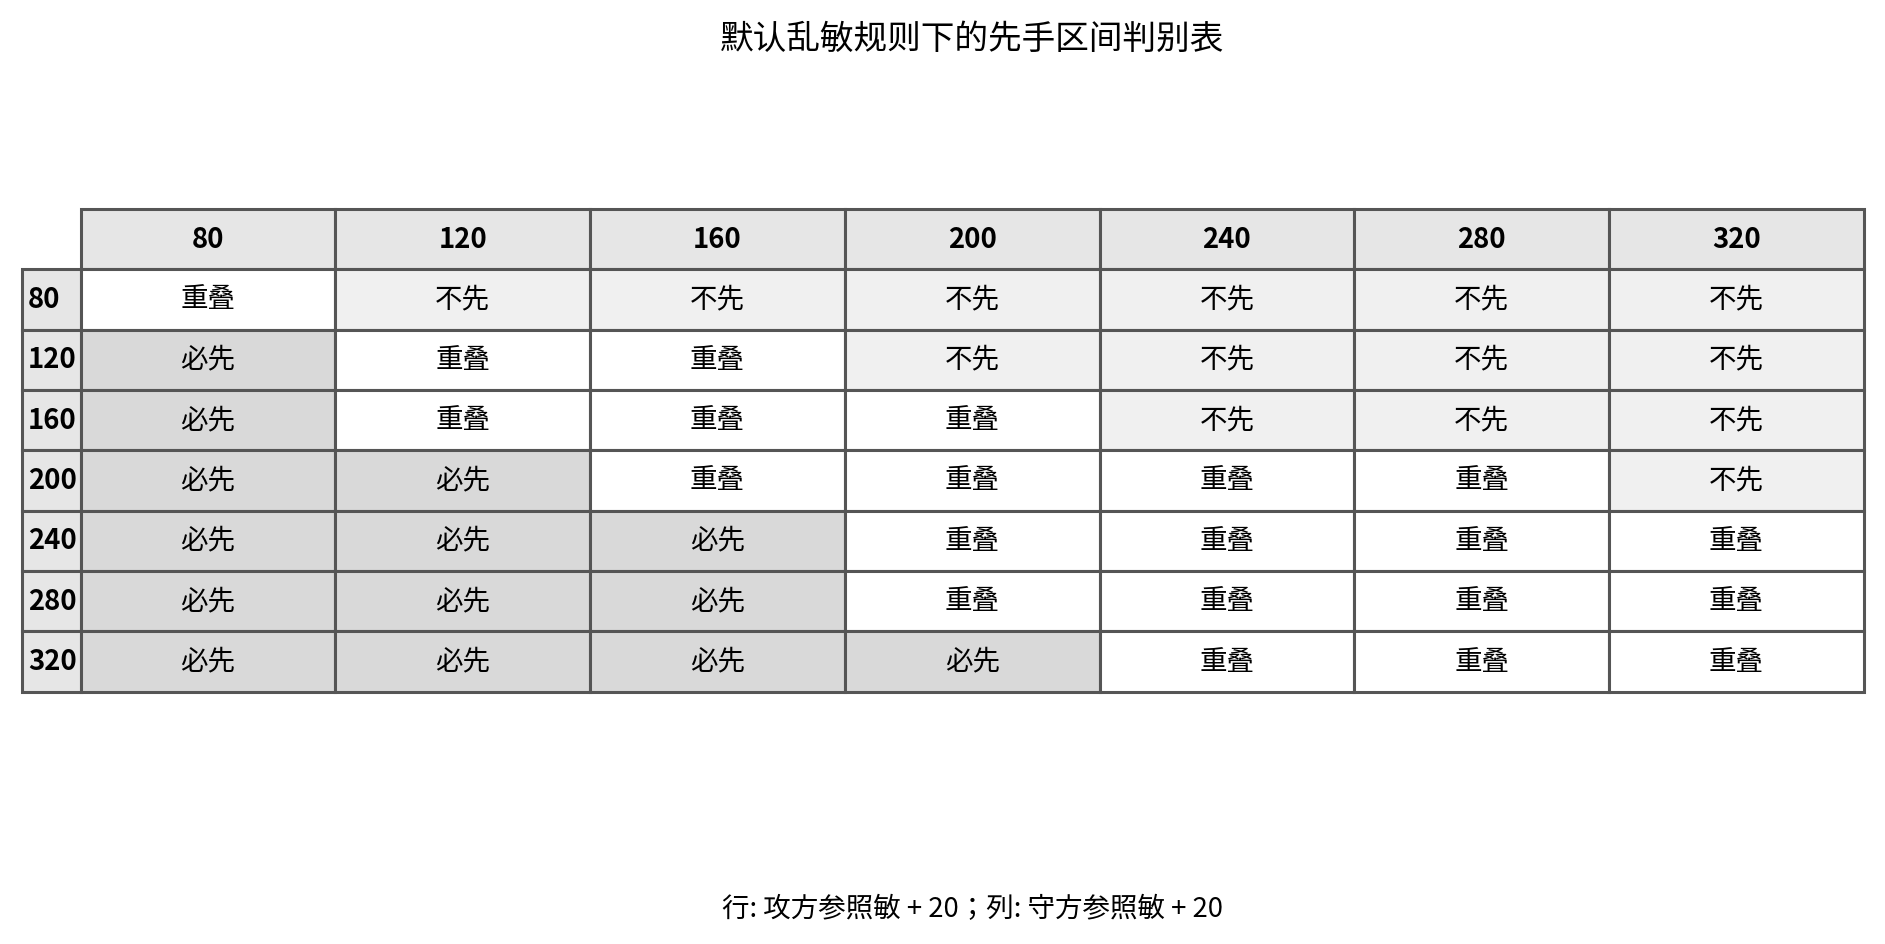
\includegraphics[width=0.88\textwidth]{figures/turn_region_table.png}
    \caption{默认乱敏规则下的先手区间判别表。图中以 $w_a=Q_{\mathrm{ref},a}+20$、$w_b=Q_{\mathrm{ref},b}+20$ 为行列，\texttt{Always} 表示攻方必定先手，\texttt{Never} 表示攻方不可能先手，\texttt{Overlap} 表示双方顺序值区间重叠，需进一步做离散随机比较。}
    \label{fig:turn-region-table}
\end{figure}

